
\chapter{Result Analysis}
\label{sec:result_analysis}

\begin{figure}[htbp]
    \centering
    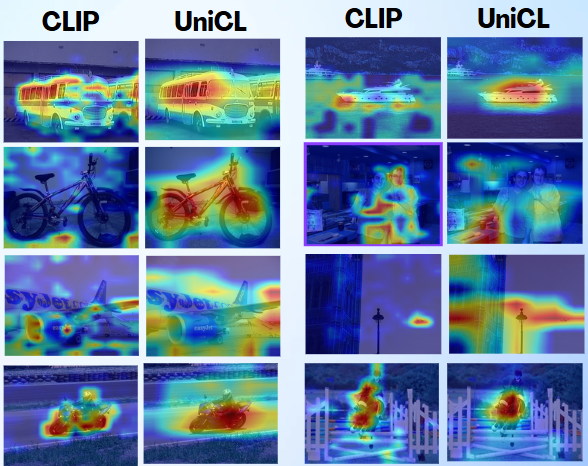
\includegraphics[width=0.8\textwidth]{clip_vs_unicl.png}
    \caption{Quantitative analysis of CAMs produced by CLIP and Swin}
    \label{fig:cam_results}
\end{figure}

\autoref{fig:cam_results} shows the comparison of the CAMs generated by CLIP \cite{vl_clip} and UniCL \cite{vl_unicl} on the Pascal VOC 2012 dataset. The results indicate that UniCL produces more accurate and detailed CAMs compared to CLIP. You can see the bicycle in second row, first two columns, CLIP even failed to detect it, while UniCL was localize it very well. The same is true for third and fourth columns of the same row, where CLIP failed to highlight the boat, but UniCL did.

Additionally, we can see in all the images that, the CAMs produced by CLIP are discontinuous and sparse, while the CAMs produced by UniCL are more continuous and dense. This indicates that UniCL is better at capturing the global context of the image.

However, we also observed that the CAMs produced by UniCL are still not perfect. It produces a lot of false positives, for example, look at the third row, last column, where it was supposed highlight an aeroplane, but it also highlighted the background. Also in some cases, like the last row, CLIP was able to trace the object boundary with better detail. This indicates that there is still room for improvement in the CAM generation process.